%------------Ejercicio 1---------------------------------------

\begin{question}
    Sea  $S$  la superficie dada por $x^{2}+ y^{2} = z$ con $z \geq 1$  y $x^{2}+ y^{2} \leq 4$  y sea  $\mathbf{F}:\mathbb{R}^{3}\rightarrow\mathbb{R}^{3}$  un campo de clase $C^{1}$ con tercer componente  nula y $\nabla \cdot \mathbf{F}$ constante 3. Calcular el flujo de  $\mathbf{F}$  a trav\'es de $S$ indicando la orientaci\'on elegida.
\end{question}

%------------Ejercicio 2---------------------------------------

\begin{question}
    Sea $\mathbf{F}(x,y,z) = (y^{2}-2xz,\;2xy+z^{3},\;3yz^{2}-x^{2}) $ y sea  $C$ una curva simple parametrizada por $\boldsymbol{\sigma}:[0,1]\rightarrow \mathbb{R}^{3}$
    tal que $\boldsymbol{\sigma}(0)=(0,0,0)$ y $\boldsymbol{\sigma}(1)=(1,2,0)$. Calcular $\int_{C} \mathbf{F}\cdot d\mathbf{s}$ indicando la orientaci\'on elegida.
\end{question}

%------------Ejercicio 3---------------------------------------

\begin{question}
    Calcular la masa del cuerpo limitado por las ecuaciones $y-x=1$ y $x^{2}+ z^{2} = 1$ en el primer octante con funci\'on de densidad $\rho$ constante.
\end{question}

%------------Ejercicio 4---------------------------------------

\begin{question}
    Sean  $k\in\mathbb{R}$,  un campo vectorial $\mathbf{F}:\mathbb{R}^{2}\rightarrow\mathbb{R}^{2}$   de clase $C^{1}$ tal que $\nabla\times \mathbf{F}=k$ y $D=\{ (x,y) \in \mathbb{R}^{2} :  |x| \leq 1 \:  ; \:   x \leq y\leq 1  \}.$ Hallar $k$ tal que $\int_{\partial D^{+}}\mathbf{F}\cdot d\mathbf{s} = 8$.
\end{question}

%------------Solucion 1---------------------------------------
\newpage
\begin{solution}
    Es \'util primero entender con qu\'e superficies y regiones se trabajar\'a.
    % \begin{center}
    % \begin{tikzpicture}
    %     \begin{axis}[
    %         view={60}{20}, % ajusta el angulo de vision
    %         xlabel=$x$,
    %         ylabel=$y$,
    %         zlabel=$z$,
    %         zmin=0, % valor minino del eje z
    %         zmax=5, % valor maximo del eje z
    %         axis lines=center, % sin caja solo ejes
    %         ticks=none, % ejes sin marcas
    %         width=10cm,
    %         height=12cm,
    %         enlargelimits=0.2, % ajuste de limite de vision
    %         domain=-3:3,
    %         y domain=-3:3,
    %         samples=30, % numero de cuadrados por simulacion (esto aumenta el tiempo de compilacion drasticamente)
    %         colormap/cool, % color
    %     ]
    %     \addplot3 [surf, opacity=0.5, draw=none, restrict z to domain=1:4, 
    %     data cs=polar, domain=0:360, y domain=0:4] (x, y, y^2);

    %     \end{axis}
    % \end{tikzpicture}
    % \end{center}
    \begin{center}
        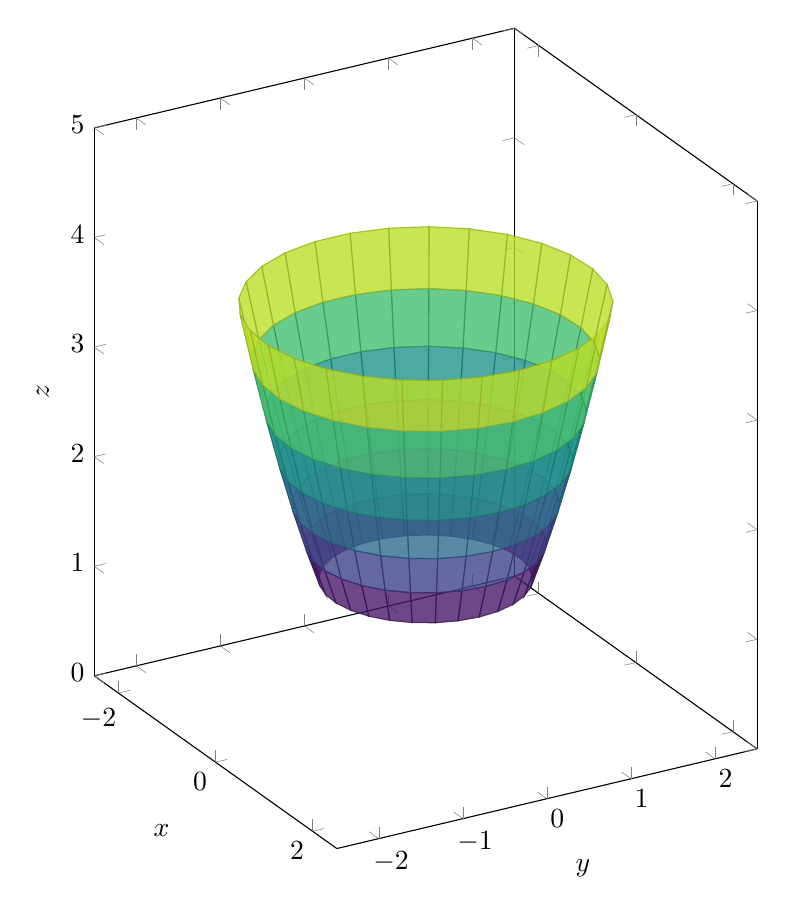
\begin{tikzpicture}
            \begin{axis}[
                    view={60}{20},
                    xlabel=$x$,
                    ylabel=$y$,
                    zlabel=$z$,
                    xmin=-2.5,
                    ymin=-2.5,
                    zmin=0,
                    xmax=2.5,
                    ymax=2.5,
                    zmax=5,
                    samples=30,
                    width=10cm,
                    height=12cm,
                    colormap/viridis,
                ]
                \addplot3 [surf, opacity=0.8, draw=none, restrict z to domain=1:4,
                    data cs=polar, domain=0:360, y domain=0:4] (x, y, y^2);
            \end{axis}
        \end{tikzpicture}
    \end{center}

    La idea es aplicar el teorema de Gauss pero  $S$ no es una superficie cerrada.   Para ello pensemos en una superficie $S'$  cerrada tal  que $S \subseteq S'.$  Definamos   $S'=S\;\cup\;S_1\;\cup\;S_2$,  donde $S_1$ y $S_2$, son las ``tapas'' del paraboloide ``cortado''.  Algebraicamente $S_1=\{(x,y,z)\in \Re^3 : x^2+y^2\le 1\;\land z=1\}$ y $S_2=\{(x,y,z)\in \Re^3 : x^2+y^2\le4\;\land z=4\}$.

    Llamando  $\Omega$  al cuerpo encerrado por $S'$ y orientando a $S'$ de manera exterior estamos en condiciones de usar el teorema de Gauss.
    \begin{gather*}
        \oiint _{S'} \mathbf{F}\cdot d\mathbf{A} =
        \iint _{S} \mathbf{F}\cdot d\mathbf{A} +
        \iint _{S_1} \mathbf{F}\cdot d\mathbf{A} +
        \iint _{S_2} \mathbf{F}\cdot d\mathbf{A}
        =\iiint _\Omega \nabla \cdot \mathbf{F}\;dV\\[.2cm]
        \iff \iint _{S} \mathbf{F}\cdot d\mathbf{A} =
        \iiint _\Omega \nabla \cdot \mathbf{F}\;dV -
        \iint _{S_1} \mathbf{F}\cdot d\mathbf{A} -
        \iint _{S_2} \mathbf{F}\cdot d\mathbf{A}\\[.2cm]
        \iff \iint _{S} \mathbf{F}\cdot d\mathbf{A} =
        I_1-I_2-I_3
    \end{gather*}

    Resolvemos el primer t\'ermino.
    \begin{align*}
        I_1=\iiint _\Omega \nabla \cdot \mathbf{F}\;dV = \iiint _\Omega3\:dV = 3\:\text{Vol}(\Omega)
    \end{align*}
    Pasando a  $\Omega$ en coordenadas cil\'indricas
    \[\begin{dcases}
            x=\rho \cos \phi \\
            y=\rho \sen \phi \\
            z=z
        \end{dcases}\] donde, $$0\leq\rho\leq \sqrt{z}\:\land\:0\leq\phi\leq 2\pi \land 1\leq z \leq 4.$$

    Entonces nos queda
    \[
        \text{Vol}(\Omega) =  \int_1^4  \int_0^{2\pi} \int_0^{\sqrt{z}}  \rho\:d\rho\:d\phi \:dz=2\pi  \int_1^4 \Big( \frac{\rho^2}{2}\Big|_0^{\sqrt{z}} \Big) \:dz =  \pi   \int_1^4   z  \:dz= \frac{15 \pi}{2}.
    \] Luego, $I_1 =  \frac{45}{2}\pi. $

    Para clacular $I_2$  debemos parametrizar $S_1$.  Sea  $D_1=\{(u,v)\in\Re^2:u^2+v^2\leq1\}$ y  sea  $$\boldsymbol{\Sigma}:D_1\subset\Re^2\to\Re^3  \mbox{ tal que }   \boldsymbol{\Sigma}(u,v)=(u,v,1).$$
    Entonces podemos reescribir
    \[
        I_2=\iint _{D_1} (\mathbf{F}\circ\boldsymbol{\Sigma})\cdot
        (\boldsymbol{\Sigma}_u\times\boldsymbol{\Sigma}_v)\:d\mathbf{A}.
    \]
    Primero calculamos las derivadas parciales de la parametrizaci\'on.
    \begin{align*}
        \boldsymbol{\Sigma}_u & =(1,0,0) \\
        \boldsymbol{\Sigma}_v & =(0,1,0)
    \end{align*}
    Entonces
    \[
        \boldsymbol{\Sigma}_u\times\boldsymbol{\Sigma}_v=(0,0,1)=\boldsymbol{\eta}.
    \]
    Podemos observar que $\boldsymbol{\eta}$ no preserva la orientaci\'on  para $S_1$ heredada  por la orientaci\'on exterior de $S'$ elegida anteriormente para poder aplicar el teorema de Gauss. En otras palabras,  $\boldsymbol{\eta}$ ``apunta''  hacia el interior de $\Omega$.  Por lo que,
    \[
        I_2=-\iint _{D_1} (\mathbf{F}\circ\boldsymbol{\Sigma})\cdot \boldsymbol{\eta}\:d\mathbf{A}.
    \]
    Calculamos el integrando aparte. Acord\'emonos que la tercer coordenada de $\mathbf{F}$ es nula. Podemos llamar
    \[
        \mathbf{F}\circ\boldsymbol{\Sigma}=(P,Q,0),
    \]
    entonces nos queda que
    \[
        (\mathbf{F}\circ\boldsymbol{\Sigma})\cdot \boldsymbol{\eta}=(P,Q,0)\cdot (0,0,1)=0.
    \]
    Por lo tanto $I_2=0$.

    Procediendo de la misma manera nos daremos cuenta que tambi\'en $I_3=0$.

    $$\therefore\;\iint _{S} \mathbf{F}\cdot d\mathbf{A}=I_1=\frac{45}{2}\pi$$
\end{solution}

%------------Solucion 2---------------------------------------

\begin{solution}
Busquemos, si existe,  una funci\'on potencial para $\mathbf{F},$ es decir, buscamos $f$ tal que $\nabla f = F.$ Para ello,  planteamos el sistema de tres ecuaciones diferenciales dado por:
\[\begin{dcases}
        y^2-2xz=f_x \\
        2xy+z^3=f_y \\
        3yz^2-x^2=f_z
    \end{dcases}\]
Entonces
\begin{equation}
    \int f_x(x,y,z)\:dx=y^2x-zx^2+g(y,z)=f(x,y,z), \label{eq:cons1}
\end{equation}
donde $g$ es la constante con respecto a $x$ producto de la integraci\'on. Derivando \eqref{eq:cons1} con respecto a $y$ obtenemos
\begin{gather*}
    f_y(x,y,z)= 2yx+g_y(y,z)\\[.2cm]
    2yx+g_y(y,z)  = 2xy+z^3 \implies g_y(y,z)=z^3\\[.2cm]
    g(y,z)=\int  g_y(y,z) \:dy =  z^3y+h(z).
\end{gather*}
Reemplazando en  la ecuaci\'on \eqref{eq:cons1},
\begin{equation}
y^2x-zx^2+z^3+h(z) =  f(x,y,z).   \label{eq:cons2}
\end{equation}

Derivando \eqref{eq:cons2} con respecto a $z$ obtenemos
\begin{gather*}
    f_z(x,y,z)=-x^2+3yz^2+h_z(z)\\
    -x^2+3yz^2+h_z(z)=3yz^2-x^2   \implies h_z(z) =0 \\[.2cm]
    h(z) = C,\quad\text{con}\;\;C\in\Re.
\end{gather*}
Por lo tanto llegamos a una familia de soluciones.
\[
    f(x,y,z)=y^2x-zx^2+z^3+C  \quad\text{con}\;\;C\in\Re
\]
Demostramos que $\mathbf{F}$ es un campo conservativo pues $\mathbf{F}=\nabla f.$ Luego, podemos calcular
\[
    \int _{\boldsymbol{\sigma}} \mathbf{F}\cdot d\mathbf{s}=
    \int _{\boldsymbol{\sigma}} \nabla f\cdot d\mathbf{s} = f(\boldsymbol{\sigma}(1))-f(\boldsymbol{\sigma}(0))=f(1,2,0)-f(0,0,0)=4.
\]
\end{solution}

%------------Solucion 3---------------------------------------

\begin{solution}
    La masa de un cuerpo de volumen $\Omega$ es
    \[
        M=\iiint_\Omega \rho\:dV.
    \]
    En este caso
    \[
        \Omega=\{(x,y,z)\in\Re^3:x^2+z^2\leq1\;\land\;y\leq1+x\; \land\;x,y,z\geq0\}.
    \]
    Conviene trabajar en coordenadas cil\'indricas. Sea
    \[\begin{dcases}
            x=r\sen\phi \\
            y=y         \\
            z=r\cos\phi.
        \end{dcases}\]
    Entonces en el nuevo sistema de coordenadas
    \[
        \Omega^*=\{(r,\phi,y)\in\Re^3:    0\leq  r\leq1\; \land\; 0 \leq y\leq1+r\sen\phi\;\land\;  0\leq\phi\leq\frac{\pi}{2}\}.
    \]

    Ahora podemos reescribir, dado que $\rho$ es constante,
    \begin{align*}
        \frac{M}{\rho} = & \iiint_{\Omega^*} r\:dy\:d\phi\:dr=\int_0^1 \int_0^{\frac{\pi}{2}} \int_0^{1+r\sen\phi} r\:dy\:d\phi\:dr \\[.2cm]
        =                & \int_0^1 \int_0^{\frac{\pi}{2}}r(1+r\sen\phi)\:d\phi\:dr=\int_0^1 \int_0^{\frac{\pi}{2}} ( r+r^2\sen\phi) \:d\phi\:dr \\[.2cm]
        =                & \int_0^1\int_0^{\frac{\pi}{2}} r\:d\phi\:dr+\int_0^1\int_0^{\frac{\pi}{2}}r^2\sen\phi\:d\phi\:dr                      \\[.2cm]
        =                & \int_0^1r\:dr\int_0^{\frac{\pi}{2}}d\phi+\int_0^1r^2\:dr\int_0^{\frac{\pi}{2}}\sen\phi\:d\phi                         \\[.2cm]
        =                & \frac{\pi}{4}+\frac{1}{2}.
    \end{align*}
    \[
        \therefore\:M=\rho\left(\frac{\pi}{4}+\frac{1}{2}\right)
    \]
\end{solution}

%------------Solucion 4---------------------------------------

\begin{solution}
    La regi\'on $D$ se grafica de la siguiente manera.

    \begin{center}
        \begin{tikzpicture}
            \begin{axis}[
                    axis lines=center,
                    axis equal,
                    xlabel=$x$,
                    ylabel=$y$,
                    xmin=-1,
                    xmax=1,
                    ymin=-1,
                    ymax=1.2,
                    xtick distance=1,
                    ytick distance=1,
                ]
                \addplot[name path=A, draw=none]{x} node[pos=0.55, right]{$y=x$};
                \addplot[name path=B, draw=none]{1};
                \addplot[fill=violet!90, opacity=0.7]fill between[of=A and B, soft clip={domain=-1:1}];
            \end{axis}
        \end{tikzpicture}
    \end{center}


    Podemos observar que $D$ es simplemente conexo y que $\partial D$ es una curva simple cerrada, por lo tanto vale el teorema de Green.
    \[
        \oint_{\partial D^+} \mathbf{F}\cdot d\mathbf{s}=\iint_D \nabla\times\mathbf{F}\cdot d\mathbf{A}=k\iint_DdA=8
    \]
    Nos quedar\'ia calcular el  $\textcolor{red}{A(D)}$,  \'area de $D$, que, por ser un tri\'angulo, se puede calcular simplemente.
    \[
        A(D) = \iint_D dA=\frac{4}{2}=2
    \]
    Entonces nos queda
    \[
        2k=8\iff k=4.
    \]
\end{solution}